\subsection{People Localization}
Our approach to achieve this task is based on the quality of the detection and painting retrieval. In fact, if our trained model correctly detect a person, in order to localize that person, we use information about the paintings detected by the model and retrieved from the database. 

\begin{figure}[h!]
    \centering
    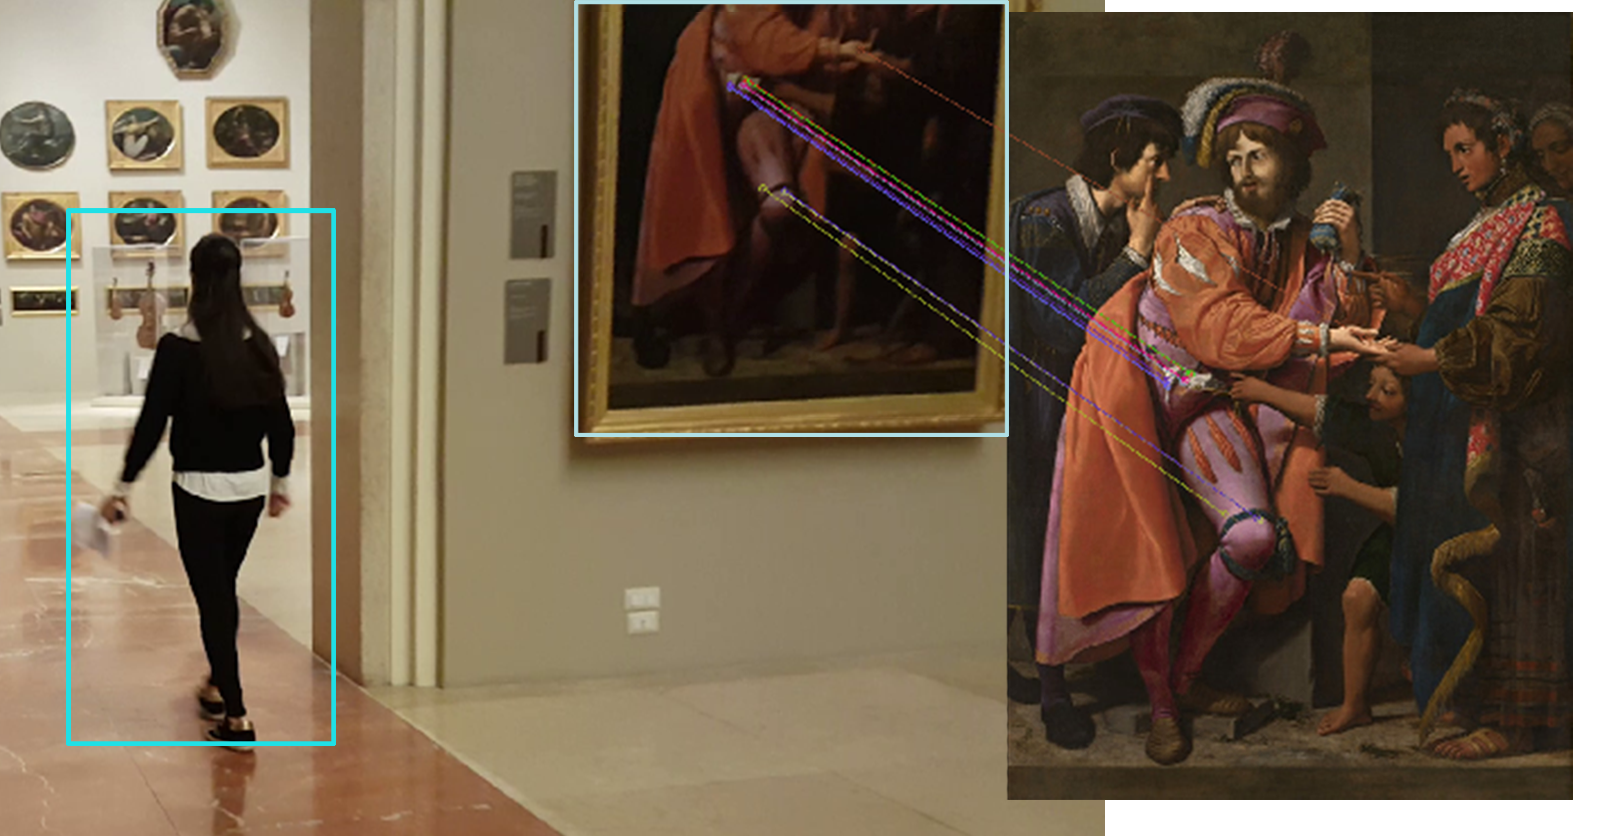
\includegraphics[width=0.4\textwidth]{pictures/people_localization/localization}
    \caption{Using detection and retrieval to localize a person.}
    \label{fig:localization}
\end{figure}

If our trained model detects a person and there is at least one painting, we retrieve that painting from the database, like the example in fig.~\ref{fig:localization}, and localize the person searching for an instance in the \emph{data.csv}, that gives us the room localization as well as the painting info.
When we have correctly localized a person, we show the Galleria Estense's map with the correct room highlighted, using a red rectangule, as shown in fig.~\ref{fig:localization_result}.

\begin{figure}[h!]
    \centering
    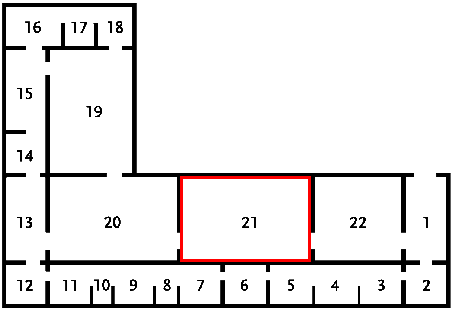
\includegraphics[width=0.3\textwidth]{pictures/people_localization/localization_result}
    \caption{Person localization.}
    \label{fig:localization_result}
\end{figure}



\subsubsection{Evaluation}
We have access to the paintings\_db, with informations about the room where each painting is located, but there are two main problems that worsen our evaluation:

\begin{enumerate}[label=\alph*)]
    \item \label{retrieval_case} The painting retrieval finds a match only in 50\% of the cases.
    \item \label{painting_other_room} We do not take into account the scenario in which the camera and the person are in a room, while a detected painting is in another room, visible through a door.
\end{enumerate}

The case \ref*{retrieval_case} is the first and only reason why our localization is not performing well, because in our evaluation we discarded all cases that match \ref*{painting_other_room} and the results are all depending on the painting retrieval, which are shown in table \ref{tab:retrieval_eval}.
